\section{Aufgabe 1 - Ampelsteuerung}
\label{sec:aufgabe-1}

Es soll eine Ampelsteuerung implementiert und getestet werden.
Die Ampel wird mithilfe von drei LEDs, in den Farben Rot, Gelb und Grün, aufgebaut.
Weiters soll die Steuerung folgende Funktionsweise implementieren:

\textbf{Phase 1} soll die Ampel auf Rot setzen.
D.h., die rote LED wird eingeschaltet.
Dieser Zustand soll vier Sekunden lang gehalten werden.

\textbf{Phase 2} soll zusätzlich zur roten LED die gelbe einschalten.
Dieser Zustand soll eine Sekunde lang gehalten werden.

\textbf{Phase 3} soll die rote sowie die gelbe LED ausschalten, während die Grüne eingeschaltet wird.
Dieser Zustand soll vier Selunden lang gehalten werden.

\textbf{Phase 4} soll die grüne LED ausschalten während die Gelbe eingeschaltet wird.
Dieser Zustand soll eine Sekunde lang gehalten werden.
Nach Ablauf der vier Sekunden soll die grüne LED erlöschen und der Ablauf bei Phase 1 neu gestartet werden.

\subsection{Materialien}
\label{subsec:A1-materialien}

\begin{table}[h]
    \centering
    \caption{Aufgabe 1 - Verwendete Materialien}
    \label{tab:a1-materialien}
    \begin{tabular}{| l | l | l |}
        \hline
        Bezeichnung & Eigenschaften & Menge \\
        \hline
        Widerstand  & $150\Omega$   & 3     \\
        & Braun - Grün - Braun - Gold & \\
        LED & Rot & 1 \\
        LED & Gelb & 1 \\
        LED & Grün & 1 \\
        Mikrocontroller & Arduino Uno R3 & 1 \\
        \hline
    \end{tabular}
\end{table}

\subsection{Vorbereitung}
\label{subsec:A1-vorbereitung}

Für den Schaltkreis müssen die Vorwiederstände für die LEDs berechnet werden.
Folgende Angaben sind bekannt.

\begin{itemize}
    \item Ausgangsspannung der Pins des Mikrocontrollers: $V_{out} = 5V$
    \item Diodenspannung der LEDs: $U_D = 2V$
    \item Diodenstrom der LEDs: $I_D = 15mA$
\end{itemize}

Zur Berechnung wird folgender Stromkreis angenommen.

\begin{figure}[h]
    \centering
    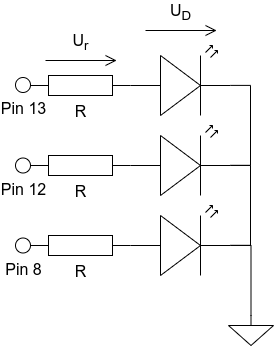
\includegraphics[height=0.4\textheight]{pictures/A1.png}
    \caption{Stromkreis A1}
    \label{fig:stromkreis-a1}
\end{figure}

Die Formel zur Berechnung des Stroms durch eine Diode ist bekannt.

\begin{equation}
    I_D =  \frac{1}{R_d} * (U - U_D) \label{eq:diodenstrom}
\end{equation}

Damit kann der benötigte Vorwiderstand berechnet werden.

\begin{equation}
    \begin{align}
        I_D =  \frac{1}{R_D} * (U - U_D) \Rightarrow \\
        R_D = \frac{1}{I_D} * (U - U_D) \\
        = \frac{1}{15mA} * (5V - 2V) \\
        = 200\Omega
    \end{align}
    \label{eq:equation-a1}
\end{equation}

Nachdem in der E6 Reihe keine $200\Omega$ Widerstände vorhanden sind, wurden $150\Omega$ gewählt.
Diese Wahl erfolgt aus folgenden Überlegungen.

\begin{enumerate}
    \item Laut angabe benötigt die LED $2V$ um zu schalten.
    \item Es existieren die Widerstände $150\Omega$ und $220\Omega$ in der E6-Reihe
    \item Bei einem Widerstand von $220\Omega$ würden, laut Gleichung \ref{eq:diodenstrom}, $I_D = \frac{3V}{220\Omega} = 13,636mA$ durch die LED fließen.
    \item Bei einem Widerstand von $150\Omega$ würden, laut Gleichung \ref{eq:diodenstrom}, $I_D = \frac{3V}{150\Omega} = 20mA$ durch die LED fließen.
\end{enumerate}
Da die Leuchtkraft einer LED von der Stromstärke abhängt und der Maximalstrom bei $20mA$ liegt, wurden $150\Omega$ gewählt.
Bei dieser Größe wird die LED bei theoretisch voller Leuchtkraft betrieben ohne die Lebensdauer markant zu verkürzen.

\subsection{Praktikumsaufgabe}
\label{subsec:praktikumsaufgabe}

Der Stromkreis wurde laut Abbildung \ref{fig:stromkreis-a1} implementiert.
Die Implementierung wird in Abbildung \ref{fig:implementierung-a1} gezeigt.

\begin{figure}[h]
    \centering
    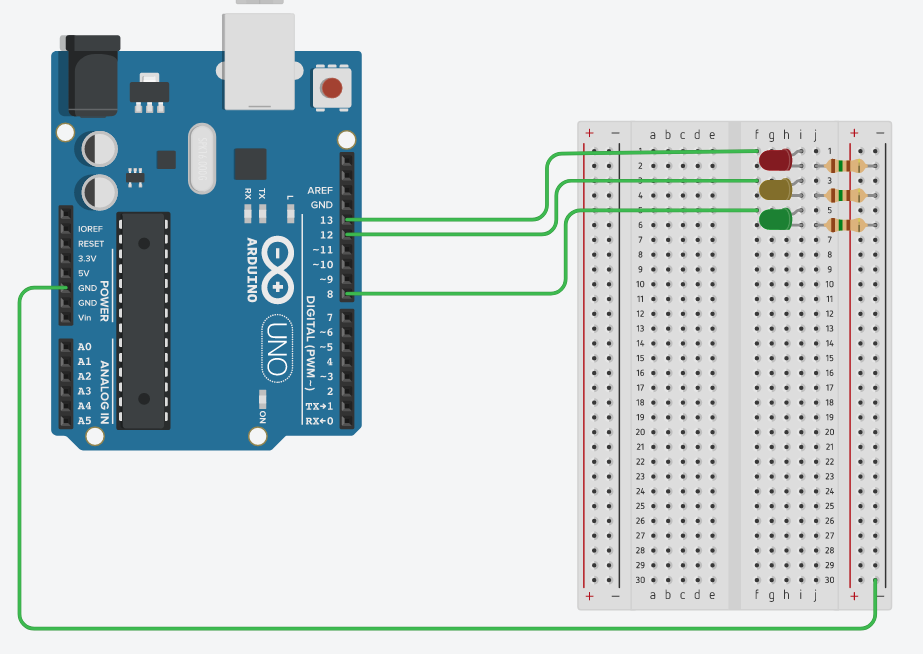
\includegraphics[width=\textwidth]{pictures/a1-praktik.png}
    \caption{Implementiert Stromkreis von Aufgabe 1}
    \label{fig:implementierung-a1}
\end{figure}

Wie in Abbildung \ref{fig:implementierung-a1} gezeigt, wurden die Pins 13, 12 und 8 gewählt.
Für die Wahl wurden die digitalen Pins herangezogen, da eine analoge Ausgabe nicht erforderlich war.
Die Pins die mit einer Tilde ($\sim$) markiert sind, sind in der Lage ein PWM-Signal zu liefern.
Da ein solches Signal nicht benötigt wird, wurden auch diese ausgeschlossen.
Von oben nach unten betrachte, wurden nun drei Pins ausgewählt, diese sind 13, 12, und 8.
Die genannten Pins werden, im Code, als digitale Output-Pins konfiguriert.

Im nachfolgendem Text wird der Programmcode der Aufgabe erläutert.
Einzelne Teile des Codes werden ausgewählt und beschrieben.
Am Ende dieser Sektion befindet sich der vollständige Programmcode.

\begin{lstlisting}[language=C,label={lst:a1-konstanten}, caption={Konstanten für Aufgabe 1}]
const int PIN_RED = 13;
const int PIN_YELLOW = 12;
const int PIN_GREEN = 8;
\end{lstlisting}

In Listing \ref{lst:a1-konstanten} werden die Pins definiert.
Durch das Anlegen von Konstanten für die Pins, kann der Code aussagekräftiger gestaltet werden.
Des weiteren entsteht dadurch die Möglichkeit, andere Pins zu verwenden, ohne den gesamtem Code durchgehen zu müssen.
Es reicht die Nummer an einer Stelle zu ändern.

\begin{lstlisting}[language=C,label={lst:a1-setup}, caption={Setup für Aufgabe 1}]
void setup()
{
  pinMode(PIN_RED, OUTPUT);
  pinMode(PIN_YELLOW, OUTPUT);
  pinMode(PIN_GREEN, OUTPUT);
}
\end{lstlisting}

In Listing \ref{lst:a1-setup} werden die Pins angelegt und konfiguriert.
Wie oben beschrieben werden die Pins als Output-Pins, d.h., als Spannungsquelle, angelegt.

\begin{lstlisting}[language=C,label={lst:a1-onoff}, caption={On- und Off Methoden für Aufgabe 1}]
void off(int pin) {
  digitalWrite(pin, LOW);
}

void on(int pin) {
  digitalWrite(pin, HIGH);
}
\end{lstlisting}

In Listing \ref{lst:a1-onoff} werden die Pins entweder ausgeschalten (LOW) oder eingeschalten (HIGH).
Durch das Verwenden dieser Methoden ist es einfacher, die Phasen zu definieren bzw., im Code zu erkennen.

\begin{lstlisting}[language=C,label={lst:a1-loop}, caption={Programmschleife für Aufgabe 1}]
void loop()
{
  off(PIN_YELLOW);
  on(PIN_RED);
  delay(4 * 1000);

  on(PIN_YELLOW);
  delay(1 * 1000);

  off(PIN_RED);
  off(PIN_YELLOW);
  on(PIN_GREEN);
  delay(4 * 1000);

  off(PIN_GREEN);
  on(PIN_YELLOW);
  delay(1 * 1000);
}
\end{lstlisting}

In Listing \ref{lst:a1-loop} werden die einzelnen Phasen implementiert.
Nach jeder Leerzeile, d.h., nach Zeile 6, 9, und 14 beginnt jeweils eine neue Phase.

Zu Beginn wird Phase 1 implementiert.
Diese Schaltet die gelbe LED, Pin 12, aus, falls vorher Phase 4 aktiv war und schaltet die rote LED, Pin 13, an.
Danach wird die $delay(x)$ Funktion aufgerufen, welche die Programmausführung für $x$ Millisekunden unterbricht.
Die Angabe von $x$ als Berechnung aus $Sekunde * 1000$ wurde gewählt, um im Code besser erkenntlich zu machen, dass es sich um Millisekunden handelt.
Der Programmfluss wird daher für vier Sekunden unterbrochen.

Dann folgt Phase 2, welche zusätzlich zur Roten auch die gelbe LED einschaltet.
Der Programmfluss wird für eine Sekunde unterbrochen.

Es folgt Phase 3.
Die Rote und die gelbe LED werden ausgeschaltet.
Die Grüne, Pin 8, wird eingeschaltet.
Der Programmfluss wird für weitere vier Sekunden unterbrochen.

Schlussendlich folgt Phase 4.
Es wird die grüne LED wieder ausgeschaltet, während die Gelbe aktiv wird.
Es folgt wieder eine Unterbrechung des Programms für eine Sekunde.
Am Ende der $loop()$ Funktion wird sie wieder von Beginn an, d.h., von Phase 1 aus, ausgeführt.


\begin{lstlisting}[language=C,label={lst:a1-programmcode}, caption={Vollständiger Programmcode für Aufgabe 1}]
const int PIN_RED = 13;
const int PIN_YELLOW = 12;
const int PIN_GREEN = 8;

void setup()
{
  pinMode(PIN_RED, OUTPUT);
  pinMode(PIN_YELLOW, OUTPUT);
  pinMode(PIN_GREEN, OUTPUT);
}

void loop()
{
  off(PIN_YELLOW);
  on(PIN_RED);
  delay(4 * 1000);

  on(PIN_YELLOW);
  delay(1 * 1000);

  off(PIN_RED);
  off(PIN_YELLOW);
  on(PIN_GREEN);
  delay(4 * 1000);

  off(PIN_GREEN);
  on(PIN_YELLOW);
  delay(1 * 1000);
}

void off(int pin) {
  digitalWrite(pin, LOW);
}

void on(int pin) {
  digitalWrite(pin, HIGH);
}
\end{lstlisting}

\subsection{Fehlerdiskussion}
\label{subsec:a1-fehlerdiskussion}

Es wurden während dieser Aufgabe keine Fehler gefunden.

\subsection{Zusammenfassung}
\label{subsec:zusammenfassung}

